\chapter{Clock Path Resilience} 

Clock Path Resilience translates into continuous and stable syntonisation and
synchronization of all the WR devices in entire WR Network. This results in very
accurate common notion of UTC in all the devices. White Rabbit has proved to
achieve sub-nanosecond accuracy over a single fibre of 10km and is expected to
achieve the accuracy of 30ns over copper \cite{TomekMSc}. The requirement by
CERN are in the range of 1$\mu s$ for most of the nodes, but a few need
accuracy of 2ns. 

A loss of UTC in WR Node can be caused by link or switch failure -- break of
clock path between the WR Timing Master and a WR Node. In order to prevent
such situation, redundancy of WR devices is introduced ensuring redundant clock
paths. However, switch-over might cause UTC instability. It is
important to minimize (eliminate) instability of UTC caused by switch-over
between redundant clock paths to avoid accuracy deterioration. The stability of
UTC is guarded in WR network by taking countermeasures to the following
phenomena:
\begin{itemize}
  \item variable external conditions, e.g. variation of temperature,
  \item temporary instability of frequency during switch-over,
  \item loss of Ethernet frames with timing information.
\end{itemize}
  
\section{Clock Distribution in WR}

Timing Information is transmitted in White Rabbit Network over Clock Path by
the means of:
\begin{itemize}
  \item Synchronous Ethernet (SyncE,\cite{SynchE}) - Physical Layer of OSI
Model.
  \item Precision Time Protocol \cite{IEEE1588} extended for White Rabbit
(WRPTP,\cite{WRPTP}) - Application Layer of OSI Model
\end{itemize}
While WRPTP uses Ethernet frames to distribute common notion of time, SyncE
uses the physical layer interface to distribute common notion of frequency. This
fact imposes the following restrictions on the Clock Path:
\begin{itemize}
  \item A White Rabbit Switch needs to have at least one of its uplinks
connected to a downlink of another White Rabbit Switch (except the Timing
Master)
  \item Timing Information (i.e. UTC notion) is sent in one direction only : 
    \begin{itemize}
      \item Network-wise : from Timing Master to the nodes.
      \item Switch-wise: from active uplink to all downlinks.
    \end{itemize}
\end{itemize}

White Rabbit Switch is designed to support Timing Path redundancy. Each switch
has two uplinks \footnote{WR Switch V3 has hardware possibility of supporting
greater number of uplinks} which can be connected to sources of Timing
Information - downlinks of another WR Switch or WR Node. A WR Switch (Node)
being the source of Timing Information is called WR Timing Master Switch (Node).
A WR Switch (Node) receiving Timing Information is called WR Timing Slave Switch
(Node). A WR Switch can be Timing Slave and Timing Master at the same time. As
mentioned before, WR Timing Slave Switch can be connected to up to two links
to up to two WR Timing Master Switches.

\begin{center}
	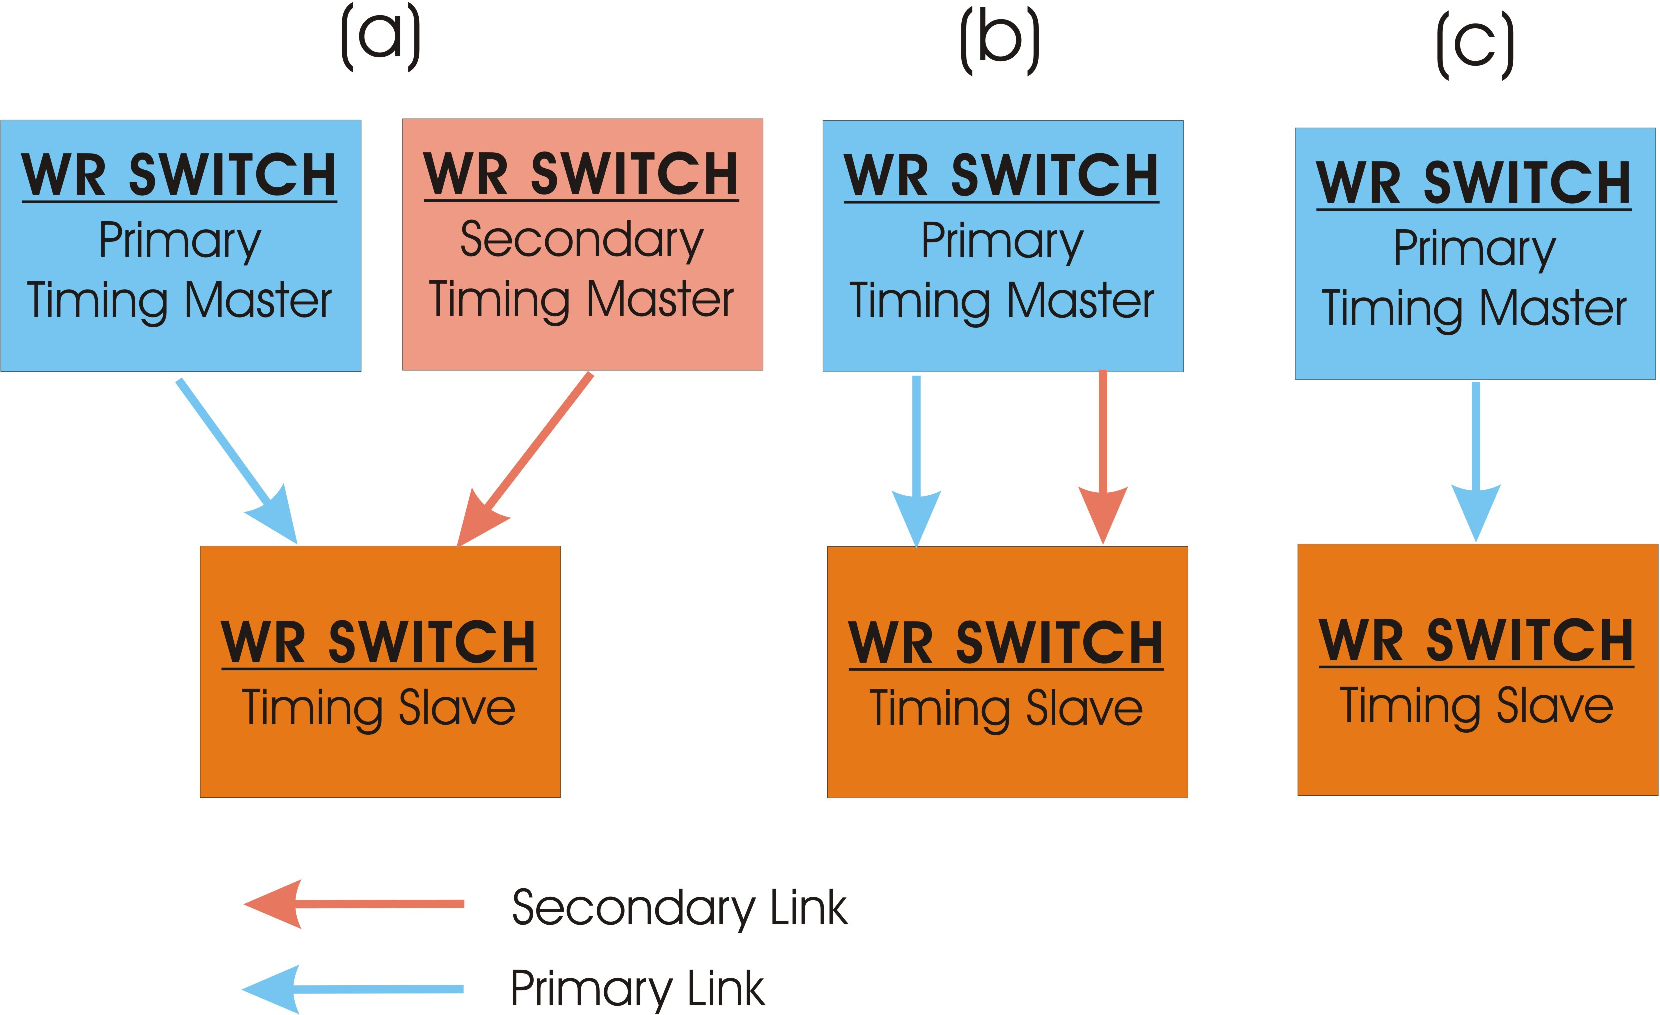
\includegraphics[scale=0.30]{robustness/timePaths.pdf}
	\captionof{figure}{Possible Timing Paths between WR Switches}
	\label{fig:timePaths}
\end{center}

Figure~\ref{fig:timePaths} depicts possible connections of a WR Switch. Clock
Path redundancy can include redundant link and switch. This happens when each
uplink of WR Timing Slave Switch is connected to independent WR Timing Master
Switch (Figure~\ref{fig:timePaths}, a). In such case we assume that independent
sources of Timing Information are synchronized with sub-nanosecond precision 
(i.e. receive the same frequency and time from GPS). It is also possible to
introduce only link redundancy as in Figure~\ref{fig:timePaths}, b). Since
redundant Timing Path is optional, the
White Rabbit network will work normally without redundancy
(Figure~\ref{fig:timePaths}, c).


\begin{center}
	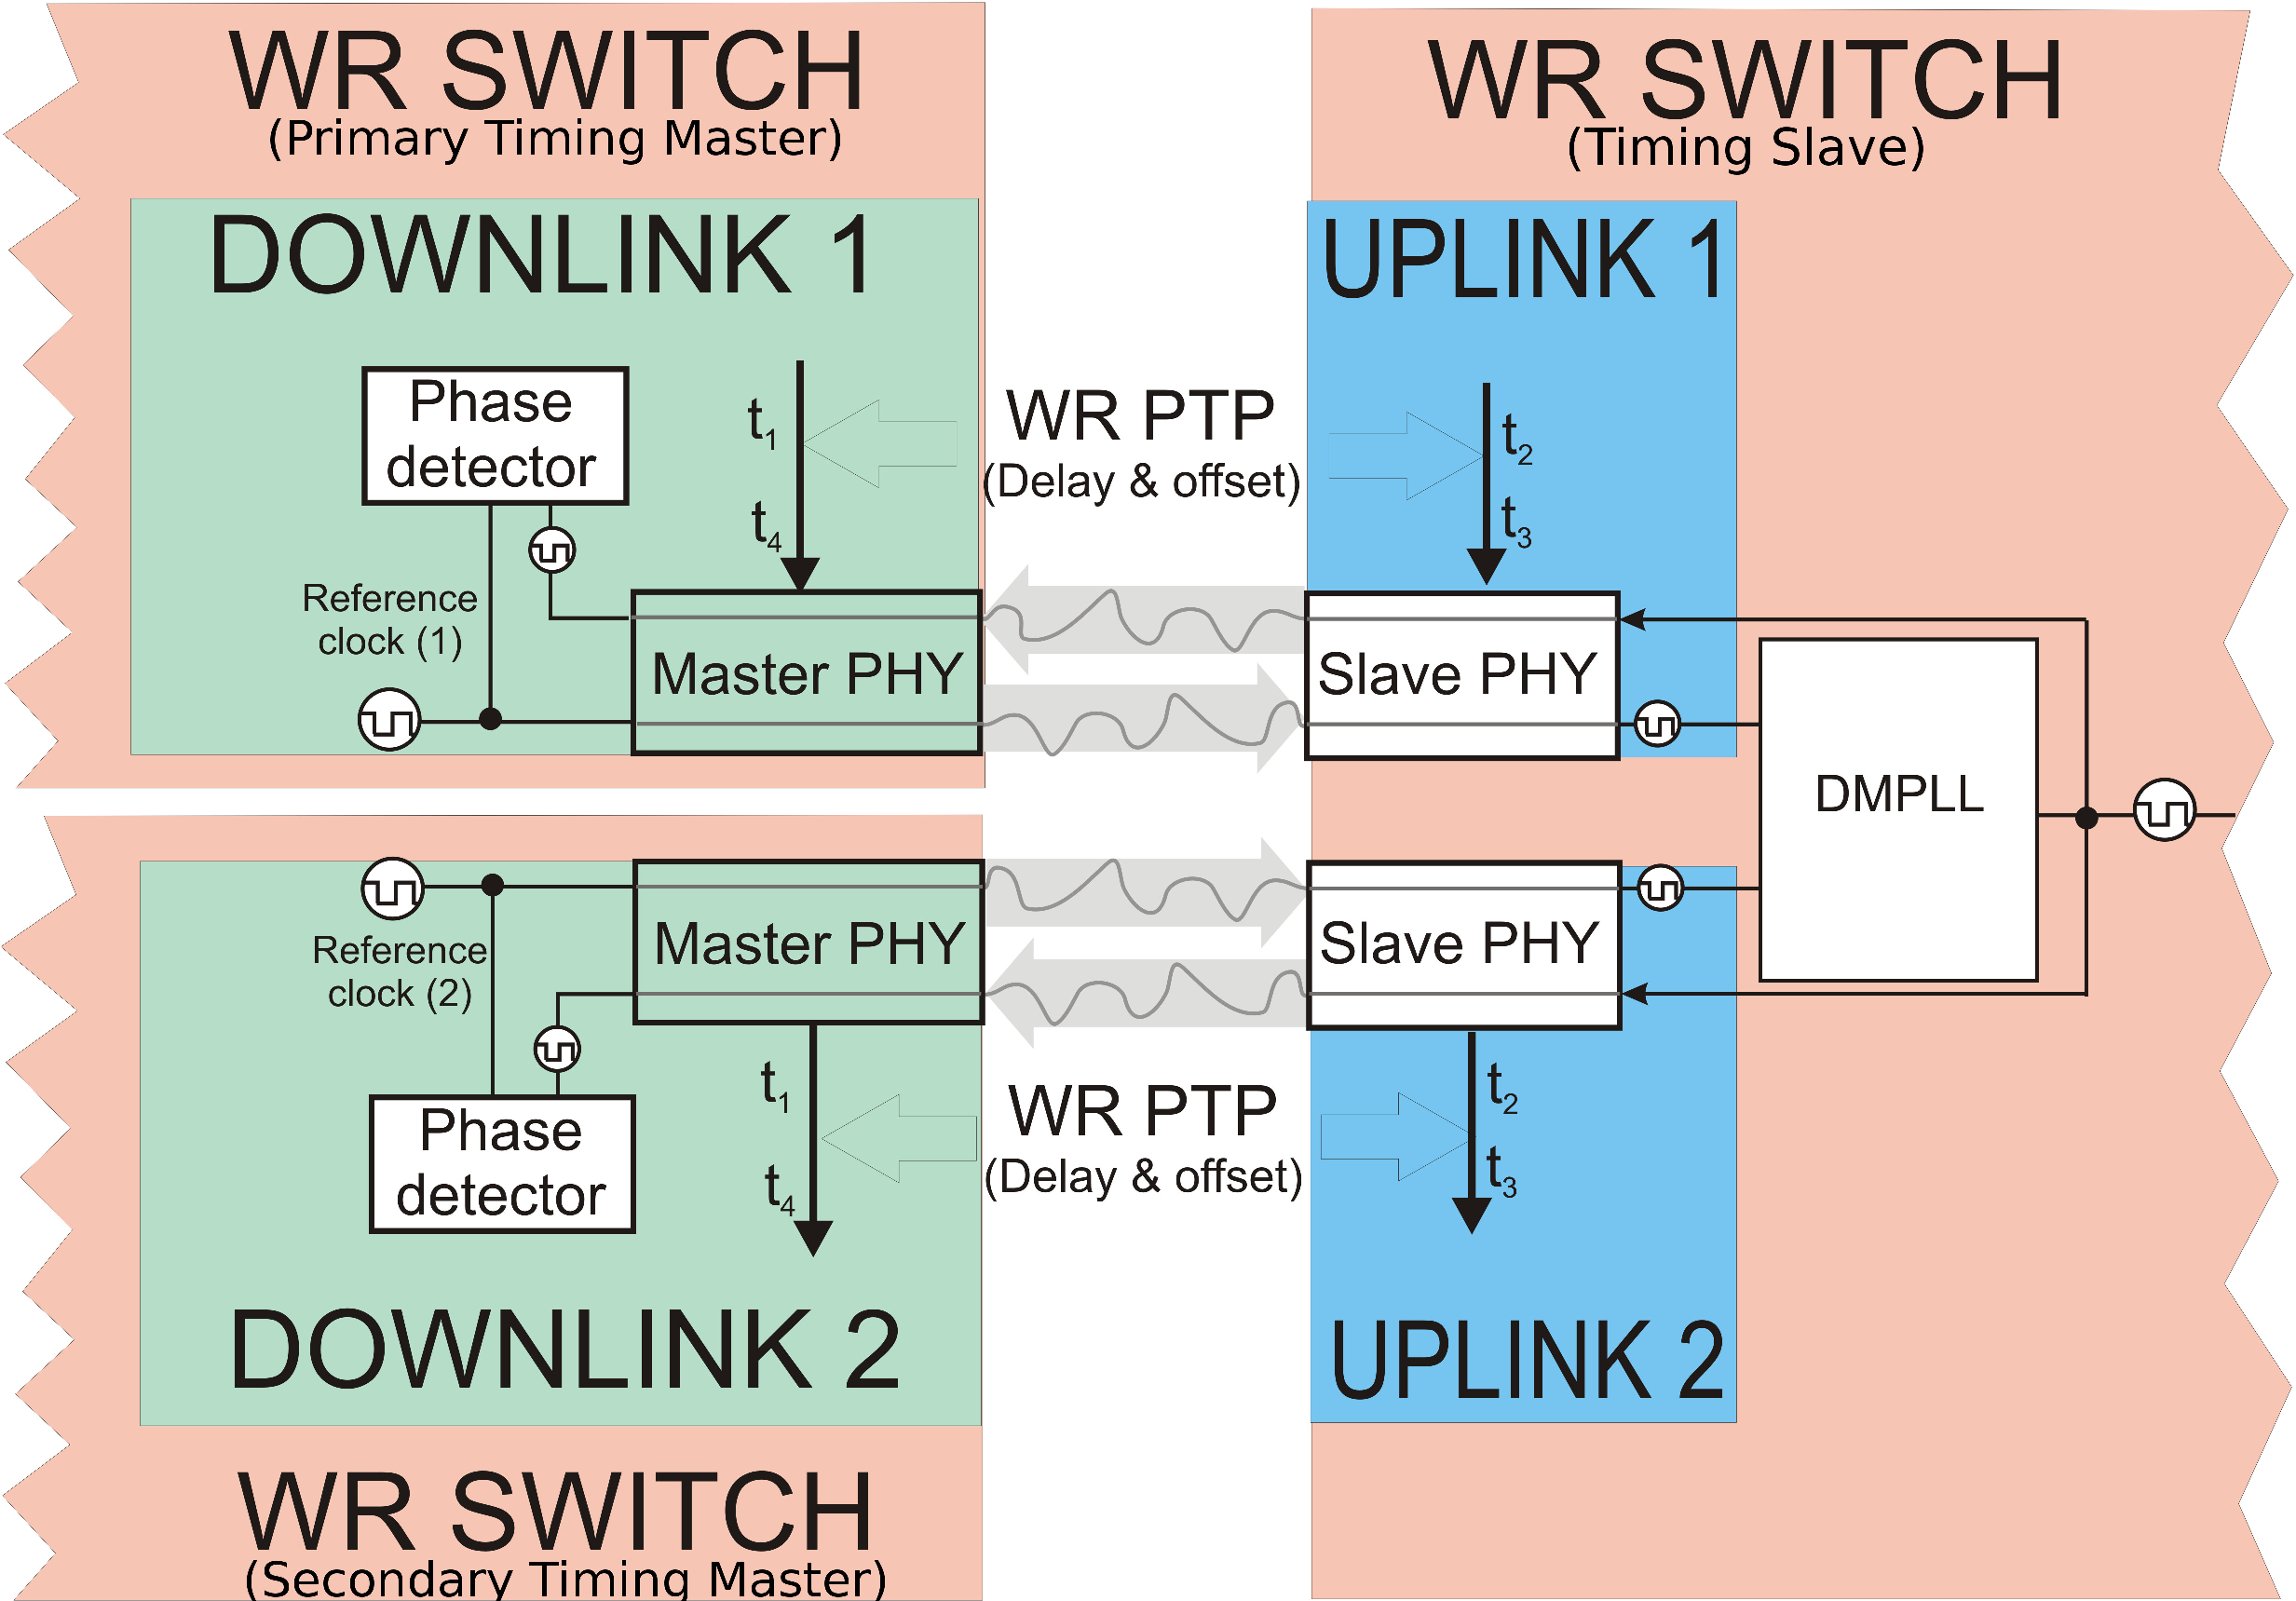
\includegraphics[scale=0.20]{robustness/layer1redundancy.pdf}
	\captionof{figure}{Clock Path Redundancy}
	\label{fig:clockRedundancy}
\end{center}

\section{Clock Path Switch-over}

As shown in Figure~\ref{fig:clockRedundancy}, uplinks retrieve frequency
sent over a link by Timing Master Switches using physical layer (SyncE). The
delay and time offset are measured by WRPTP. At any give moment,
timing and frequency from single uplink are used for syntonization and
synchronization of the local clock to Timing Master's UTC.

Since two separate technologies are used to retrieve UTC, there are two
possible sources of instability during clock path switch-over: SyncE and WRPTP.

\subsubsection{SyncE}

A detailed description of frequency recovery in WR Switch (i.e. description of
Helper PLL and Main PLL) can be found in \cite{TomekMSc}. The most important
feature of the implementation is the fact that at any given time, phase is
measured and compensated on all the uplinks simultaneously. As a result, in
theory, the switch-over between redundant links should be unnoticeable
frequency-wise introducing no accuracy deterioration. This, however, needs to be
proved by extensive tests.

\subsubsection{WRPTP} 

In principle, the values of offset and delay are measured by WRPTP on all
uplinks at any time. The values from an arbitrary uplink, which is called
Primary Link, are used to synchronize the local clock. But, the values from the
backup uplink(s) are always ready. The Primary Links should be the same
for SyncE and WRPTP. If a failure of Primary Link is detected, the values of
offset and delay available for the Secondary Linkare used. Therefore, the
switch-over WRPTP-wise is considered seemless, however, tests must be conducted
to confirm this.

The choice of the Primary Link is arbitrary. As soon as it is detected that the
Primary Link is down, the Secondary Link becomes Primary.


\section{Variable external conditions vs. stability}

The stability of UTC in WR Timing Slaves is mainly endangered by variation of
temprature which causes changes of signal propagation speed in physical medium. 
The propagation delay is measured using WRPTP which updates the values of delay
and offset with each PTP message exchange. The responsiveness of the system to
temperature variation can be controlled with frequency of PTP message exchange.
Since the gradient of temperature changes, in normal circumstances, is low (few
degrees per hour) and the frequency of PTP messages exchange much higher, it
shall not introduce deterioration of UTC accuracy. Test of propagation delay
variation is described in \cite{TomekMSc} and shown in \cite{WRdemo}. 

\section{Loss of Ethernet frames with timing information}

PTP is designed to tolerate loss of PTP-specific messages on the
communication channel. It is done through timeouts. If an operation (e.g.:
delay and offset measurement) is disrupted due to PTP message loss, the
operation is repeated after time interval elapsed -- the message is
re-sent.

White Rabbit extension to PTP (WRPTP) employs the same strategy during
WR-specific operation of White Rabbit Link Setup (see \cite{WRPTP}). In the case
of message loss, operation is repeated and the lost message is re-sent (up to a
number of times). Additionally, WRPTP is much more tolerant to a loss of
multiple messages exchanged to measure delay and offset. Unlike in
standard PTP, these measurements are used only for synchronization
(syntonization is done through SyncE). Therefore, once the synchronization is
achieved (delay and offset measured) at the beginning of the connection (e.g.:
after plugging in the physical link), the values change almost solely due
to external conditions. The rate of measurements (exchange of messages) is
supposed to be much higher then the changes of physical parameters caused by
external conditions. Therefore, even a loss of a few consecutive PTP messages
should have no influence on the WRPTP performance.
